\documentclass[aspectratio=169,11pt]{beamer}
\usetheme{default}
\usecolortheme{default}

\setbeamertemplate{navigation symbols}{}
\setbeamertemplate{footline}[frame number]

\usepackage{amsmath}
\usepackage{booktabs}
\usepackage{graphicx}
\usepackage{tikz}
\usetikzlibrary{shapes,arrows,positioning,calc}

% Small citation macro
\newcommand{\citeslide}[1]{\hfill{\footnotesize [#1]}}

\title{BZ Reaction-Diffusion Computing}
\subtitle{A Real-Chemistry Path for Project~11}
\author{Srivijayesh Venugopal}
\date{Cranfield IRP 2025-26 --- Supervisor Meeting, 15 July 2026}

\begin{document}

% ---------------------------------------------------------------------
\begin{frame}
\titlepage
\end{frame}

% ---------------------------------------------------------------------
\begin{frame}{What this meeting is for}

\begin{enumerate}
    \item Recap where we have been (wave computing \textrightarrow{} CRNs \textrightarrow{} DNA).
    \item Explain why DNA strand-displacement is not the right vehicle for this project.
    \item Propose a Belousov-Zhabotinsky (BZ) reaction-diffusion direction with trainable geometry.
    \item Agree on the next concrete simulation target.
\end{enumerate}

\vspace{0.5cm}
\centering
\textbf{Goal: pick a single direction we can simulate and write up in the remaining time.}

\end{frame}

% ---------------------------------------------------------------------
\begin{frame}{Project 11: the original premise}

\textit{``Physical fluid-based neural computation''} \citeslide{Project list, Cranfield GDP 2025-26}

\vspace{0.4cm}
Two design goals:
\begin{itemize}
    \item \textbf{Continuity:} processing occurs across the whole architecture space, not at discrete nodes.
    \item \textbf{Parallelism:} non-reactive fluid streams allow multiple independent inference processes simultaneously.
\end{itemize}

\vspace{0.3cm}
Three intended phases:
\begin{enumerate}
    \item Model a controllable physical space (reactor / microfluidic geometry).
    \item Train control units (flow rates, valve timing, \textbf{mixing topology}).
    \item Benchmark against silicon neural networks.
\end{enumerate}

\vspace{0.3cm}
\centering
\textbf{The trainable parameter is the \underline{geometry or control field}, not just rate constants.}

\end{frame}

% ---------------------------------------------------------------------
\begin{frame}{Journey so far}

\begin{table}
\centering
\small
\begin{tabular}{p{3.0cm}p{5.0cm}cc}
\toprule
\textbf{Direction} & \textbf{What it is} & \textbf{Spatial?} & \textbf{Trainable geometry?} \\
\midrule
Acoustic porous medium & Sound waves in structured solid & Yes & Pore geometry \\
Well-mixed CRN & Mass-action ODEs & No & Rate constants only \\
DNA WTA & Strand-displacement in test tube & No & Strand concentrations \\
\textbf{BZ + geometry} & \textbf{Excitable chemical waves in channels} & \textbf{Yes} & \textbf{Channel layout + field} \\
\bottomrule
\end{tabular}
\end{table}

\vspace{0.3cm}
\centering
The BZ + geometry route is the only one that keeps \textbf{both} the spatial continuity \textbf{and} the trainable-architecture idea of Project~11.

\end{frame}

% ---------------------------------------------------------------------
\begin{frame}{What we built: a well-mixed trainable CRN}

Dack-style recurrent neural CRN \citeslide{Dack et al., 2026}:
\begin{align*}
    \frac{dX_i}{dt} &= \beta_i + X_i \sum_j \alpha_{ij} Y_j \\
    \mu \frac{dY_j}{dt} &= \gamma + \theta_j Y_j + Y_j \sum_i \omega_{ji} X_i - Y_j^2
\end{align*}

\vspace{0.2cm}
\begin{itemize}
    \item Fast perceptrons $Y_j$ act as a smooth ReLU layer.
    \item Executive species $X_i$ hold inputs and output.
    \item Trained with L-BFGS-B; recurrent version solves XOR cleanly.
\end{itemize}

\vspace{0.2cm}
\centering
\textbf{Result:} a proof-of-concept that trainable chemical kinetics can learn a non-linear function.

\end{frame}

% ---------------------------------------------------------------------
\begin{frame}{Result: recurrent RNCRN solves XOR}

\centering
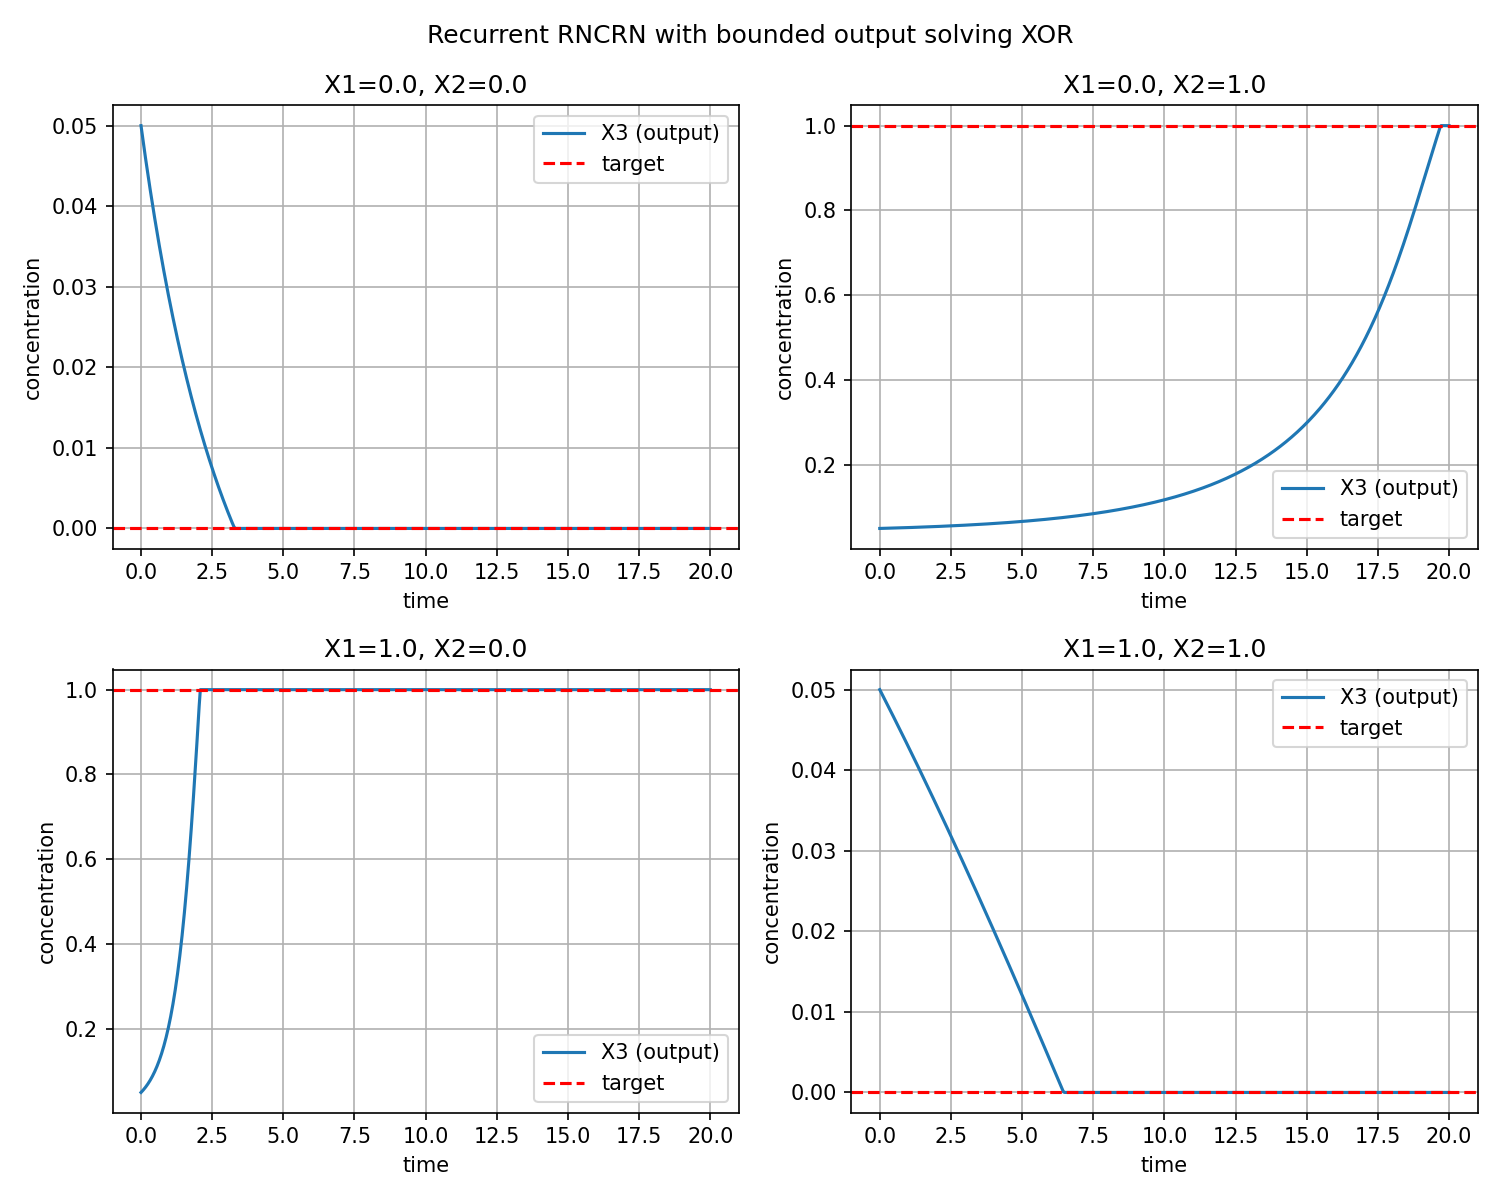
\includegraphics[width=0.60\textwidth]{../Analysis/dack_rncrn_xor_recurrent_bounded_results.png}

\vspace{0.3cm}
\begin{table}
\centering
\begin{tabular}{cc|cc}
\toprule
$X_1$ & $X_2$ & target & predicted $X_3$ \\
\midrule
0 & 0 & 0 & 0.0000 \\
0 & 1 & 1 & 1.0000 \\
1 & 0 & 1 & 1.0000 \\
1 & 1 & 0 & 0.0000 \\
\bottomrule
\end{tabular}
\end{table}

\end{frame}

% ---------------------------------------------------------------------
\begin{frame}{Why we looked at DNA, and why it is not the right fit}

Cherry \& Qian 2018 \citeslide{Cherry \& Qian, Nature 2018}: a beautiful DNA WTA neural network.

\vspace{0.2cm}
\begin{itemize}
    \item Weights = initial concentrations of DNA strands.
    \item Computation = strand-displacement reactions in a well-mixed test tube.
    \item They classify 100-bit MNIST patterns into 9 digits.
\end{itemize}

\vspace{0.3cm}
\textbf{Why this drifts away from Project~11:}
\begin{itemize}
    \item It is \textbf{well-mixed}, not spatially continuous.
    \item The trainable parameters are \textbf{molecular concentrations}, not geometry or flow.
    \item It requires specialist DNA sequence design and thermodynamics knowledge.
    \item It does not exploit the ``parallel independent inference streams'' idea.
\end{itemize}

\end{frame}

% ---------------------------------------------------------------------
\begin{frame}{Proposal: BZ reaction-diffusion computing in structured geometry}

Use a BZ-like excitable medium inside a designed channel network.

\vspace{0.3cm}
\begin{center}
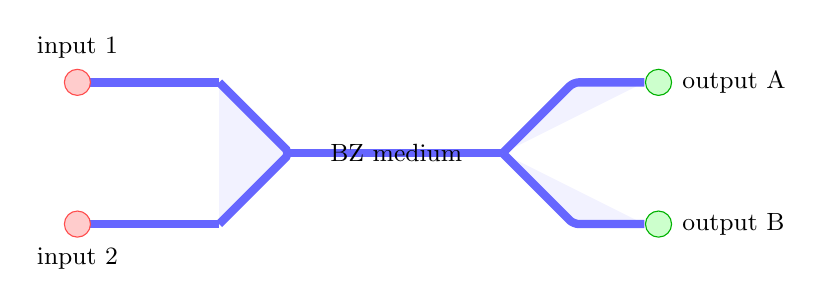
\begin{tikzpicture}[scale=0.9,
    channel/.style={draw=blue!60, line width=3pt, rounded corners=2pt, fill=blue!5},
    input/.style={draw=red!70, fill=red!20, circle, minimum size=6pt},
    output/.style={draw=green!70!black, fill=green!20, circle, minimum size=6pt},
    block/.style={draw=black!60, fill=black!15, rectangle, minimum width=12pt, minimum height=12pt}]

% Input channels
\draw[channel] (0,2) -- (2,2);
\draw[channel] (0,0) -- (2,0);

% Active region / mixer
\draw[channel] (2,2) -- (3,1) -- (2,0);
\draw[channel] (3,1) -- (6,1);

% Output branches
\draw[channel] (6,1) -- (7,2) -- (8,2);
\draw[channel] (6,1) -- (7,0) -- (8,0);

\node[input] at (0,2) {};
\node[input] at (0,0) {};
\node[output] at (8.2,2) {};
\node[output] at (8.2,0) {};

\node[right] at (8.4,2) {\small output A};
\node[right] at (8.4,0) {\small output B};
\node[above] at (0,2.2) {\small input 1};
\node[below] at (0,-0.2) {\small input 2};
\node at (4.5,1) {\small BZ medium};
\end{tikzpicture}
\end{center}

\vspace{0.3cm}
\textbf{Idea:} excitation waves enter at the left; their interference, annihilation, and routing inside the geometry determine which output fires.

\end{frame}

% ---------------------------------------------------------------------
\begin{frame}{How does a BZ medium compute?}

Three paradigms:

\vspace{0.3cm}
\begin{enumerate}
    \item \textbf{Wave collision logic:} pulses annihilate or merge at junctions \textrightarrow{} AND, OR, XOR gates \citeslide{Adamatzky \& De Lacy Costello, 2002; T\'oth \& Showalter, 1995}.
    \item \textbf{Pattern-as-state:} final spatial pattern encodes the answer; read out at fixed probe locations.
    \item \textbf{Trainable field:} optimize catalyst density or excitability map so input patterns evolve to the correct output patterns.
\end{enumerate}

\vspace{0.3cm}
For Project~11, we combine 2 and 3: \textbf{designed geometry guides the waves; trainable parameters tune the response.}

\end{frame}

% ---------------------------------------------------------------------
\begin{frame}{Candidate RD models}

\begin{table}
\centering
\footnotesize
\begin{tabular}{p{2.8cm}p{4.0cm}cc}
\toprule
\textbf{Model} & \textbf{What it does} & \textbf{Real chemistry?} & \textbf{Easy to simulate?} \\
\midrule
Gray-Scott & Spots / stripes from activator-inhibitor kinetics & No (model) & Yes \\
Belousov-Zhabotinsky & Oscillating excitable waves & Yes & Moderate \\
Iodate--arsenous acid & Simpler excitable waves than BZ & Yes & Moderate \\
FitzHugh-Nagumo & Nerve-like pulse propagation & No (model) & Yes \\
Turing patterns & Stationary activator-inhibitor patterns & Yes & Yes \\
\bottomrule
\end{tabular}
\end{table}

\vspace{0.3cm}
\textbf{Recommendation:} use the \textbf{Oregonator reduction of BZ} for the core physics (real chemistry, excitable waves, proven logic-gate literature), add channel geometry, then train wall positions or the light-suppression field $\phi(x,y)$.

\end{frame}

% ---------------------------------------------------------------------
\begin{frame}{Model: Oregonator reduction of BZ chemistry}

The Oregonator captures the BZ reaction's excitable dynamics with two
concentration fields:
\begin{align*}
    \frac{\partial u}{\partial t} &= D_u \nabla^2 u + \frac{1}{\varepsilon}\left[ u - u^2 - (f v + \phi)\frac{u-q}{u+q} \right] \\
    \frac{\partial v}{\partial t} &= D_v \nabla^2 v + u - v
\end{align*}

\vspace{0.2cm}
\begin{itemize}
    \item $u$ $\sim$ HBrO$_2$ (activator),
    \item $v$ $\sim$ oxidised catalyst Ce(IV) (recovery variable),
    \item $q$, $f$, $\varepsilon$ = kinetic parameters from the FKN mechanism,
    \item $\phi(x,y)$ = light-induced suppression (a spatially tunable field).
\end{itemize}

\vspace{0.2cm}
This is still a reduction, but it is chemically grounded and produces the target waves, annihilation, and diffraction we need for computing.

\end{frame}

% ---------------------------------------------------------------------
\begin{frame}{First result: Oregonator BZ waves}

We have a working 2D Oregonator solver.  A small excited seed produces
circular target waves; two seeds produce counter-propagating waves that
interact and suppress each other where they meet.

\vspace{0.2cm}
\begin{columns}
\begin{column}{0.49\textwidth}
\centering
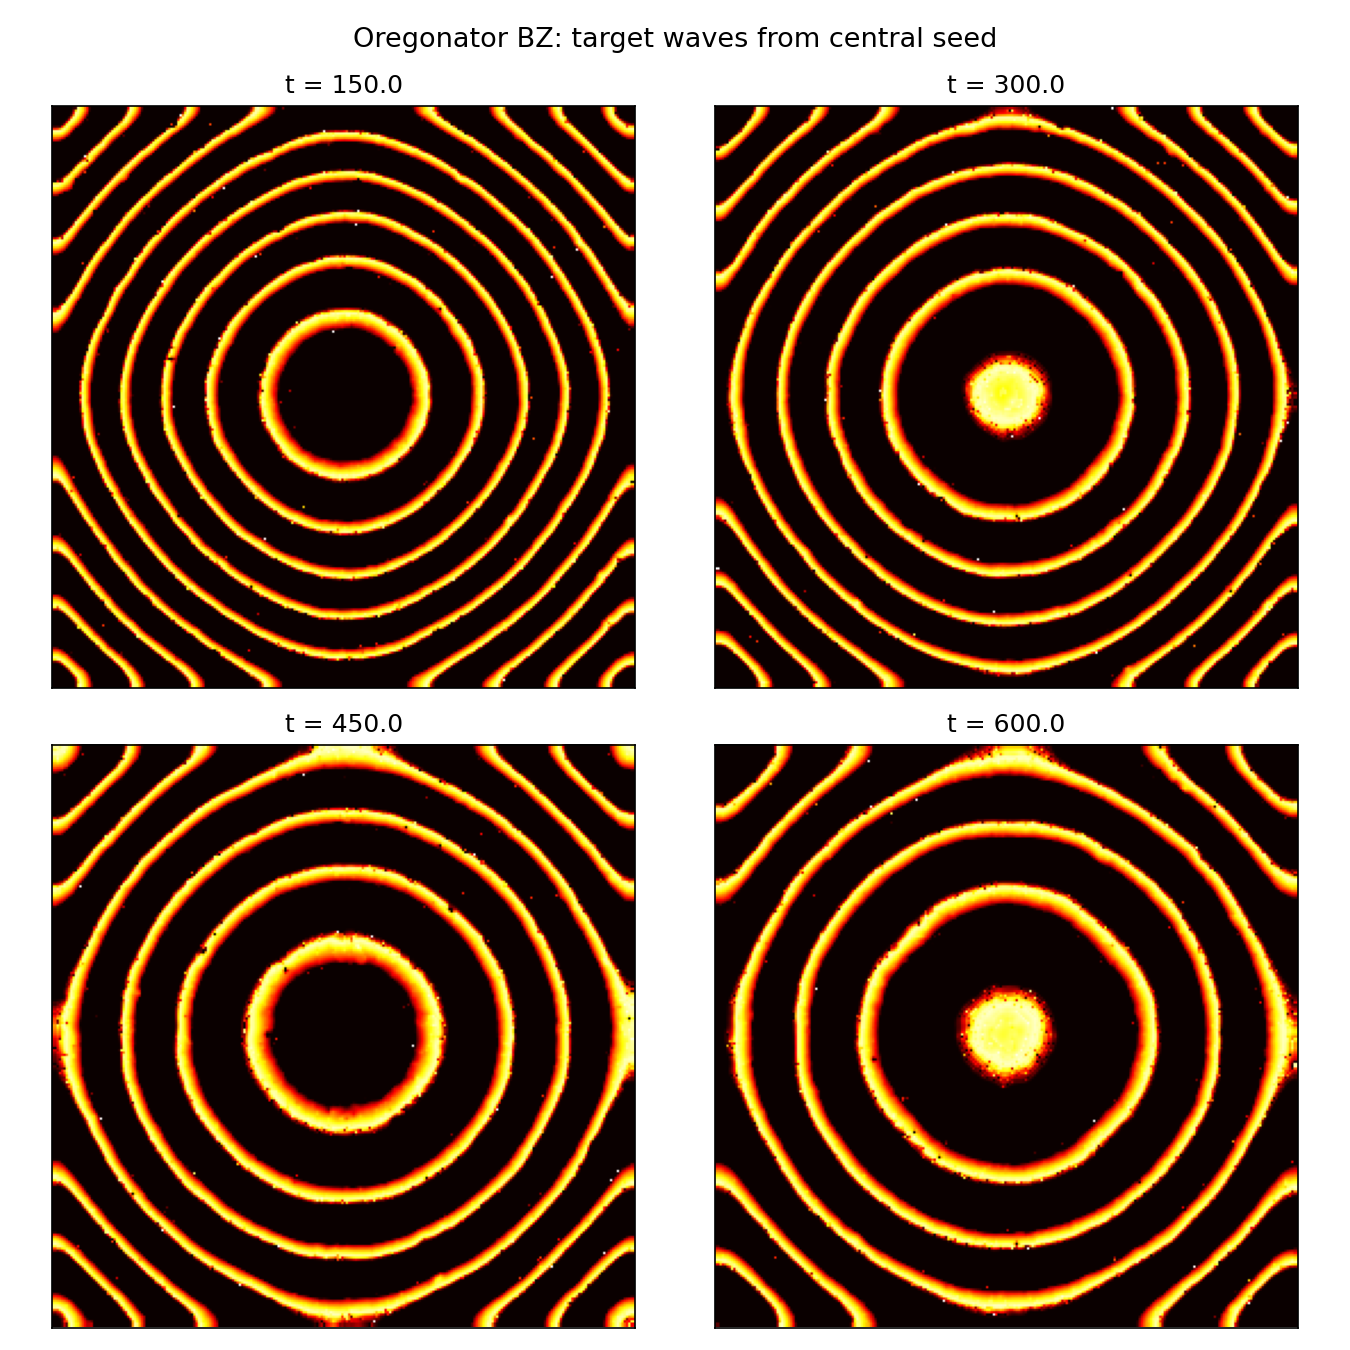
\includegraphics[width=\textwidth]{../Analysis/oregonator_target.png}
\\
{\footnotesize Target waves}
\end{column}
\begin{column}{0.49\textwidth}
\centering
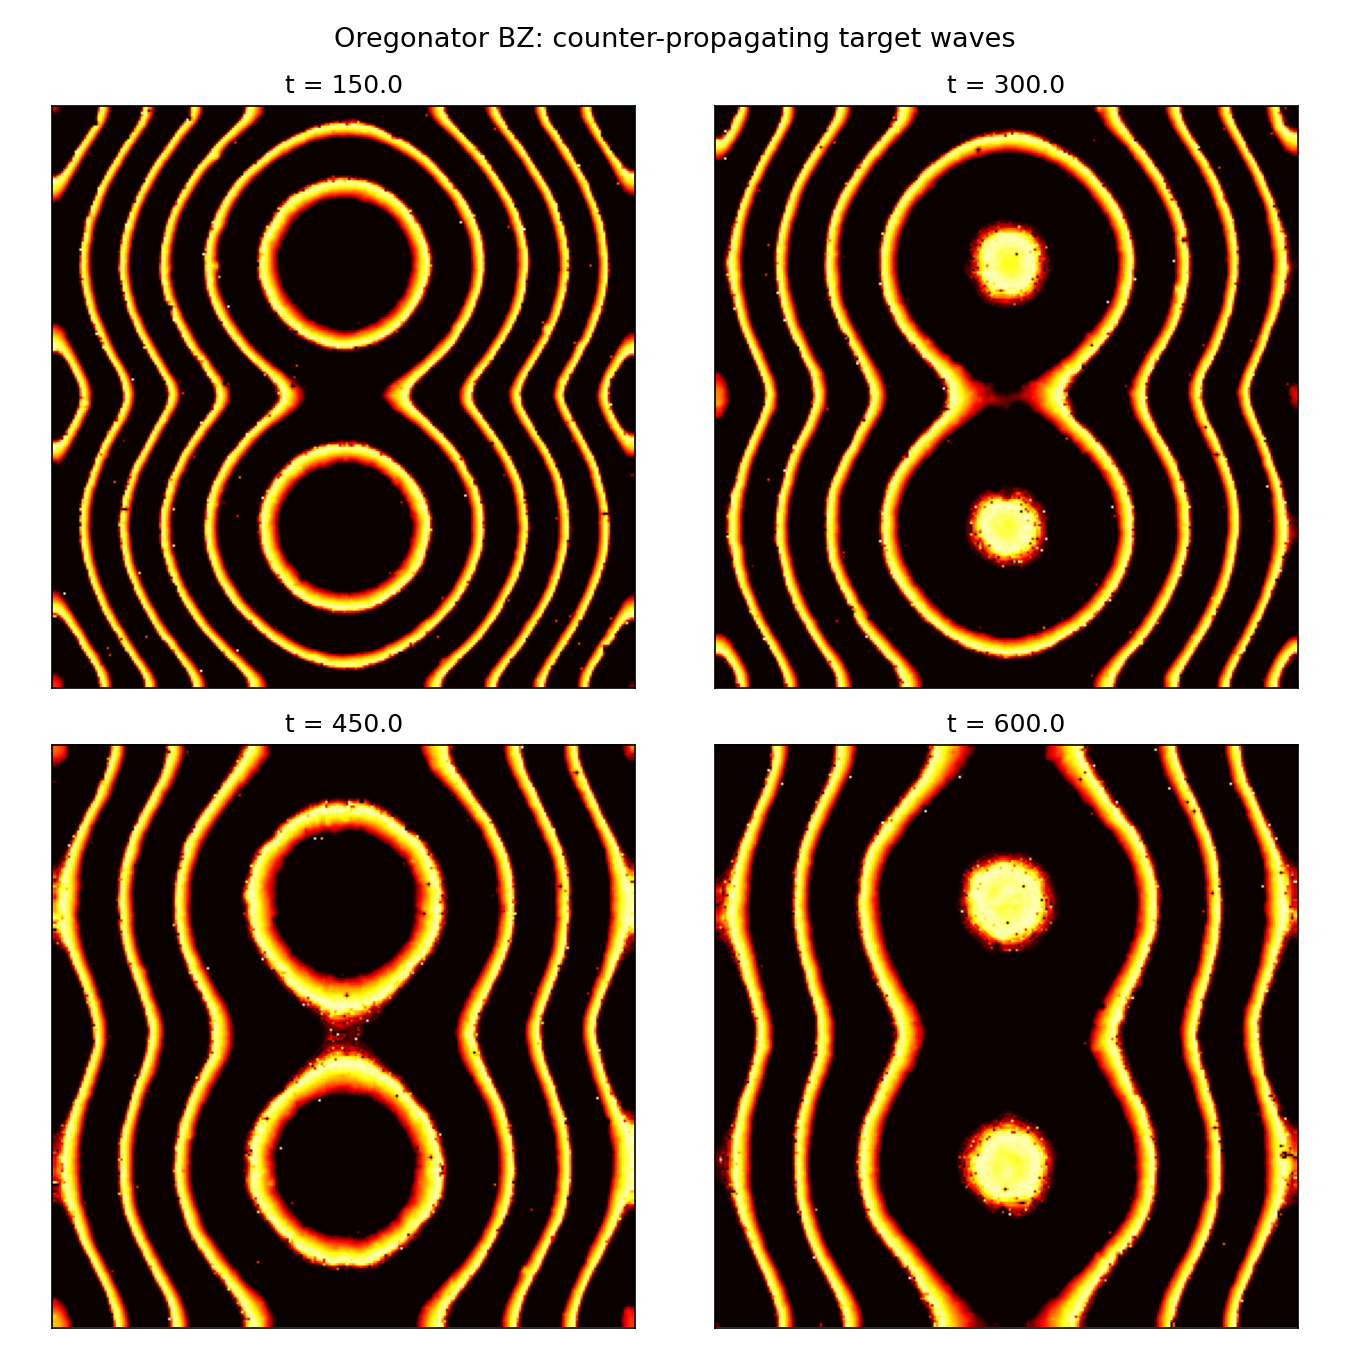
\includegraphics[width=\textwidth]{../Analysis/oregonator_collision.png}
\\
{\footnotesize Counter-propagating waves}
\end{column}
\end{columns}

\vspace{0.2cm}
\footnotesize
This is not yet a trained computer, but it proves the medium supports the propagating, colliding pulses that underpin BZ logic gates.

\end{frame}

% ---------------------------------------------------------------------
\begin{frame}{Wave routing by geometry: diffraction through a gap}

A no-flux wall with a small gap blocks most of the wave but lets a
fragment through; the fragment spreads out on the far side.  This is the
prototype for channel-controlled routing in Project~11.

\vspace{0.3cm}
\centering
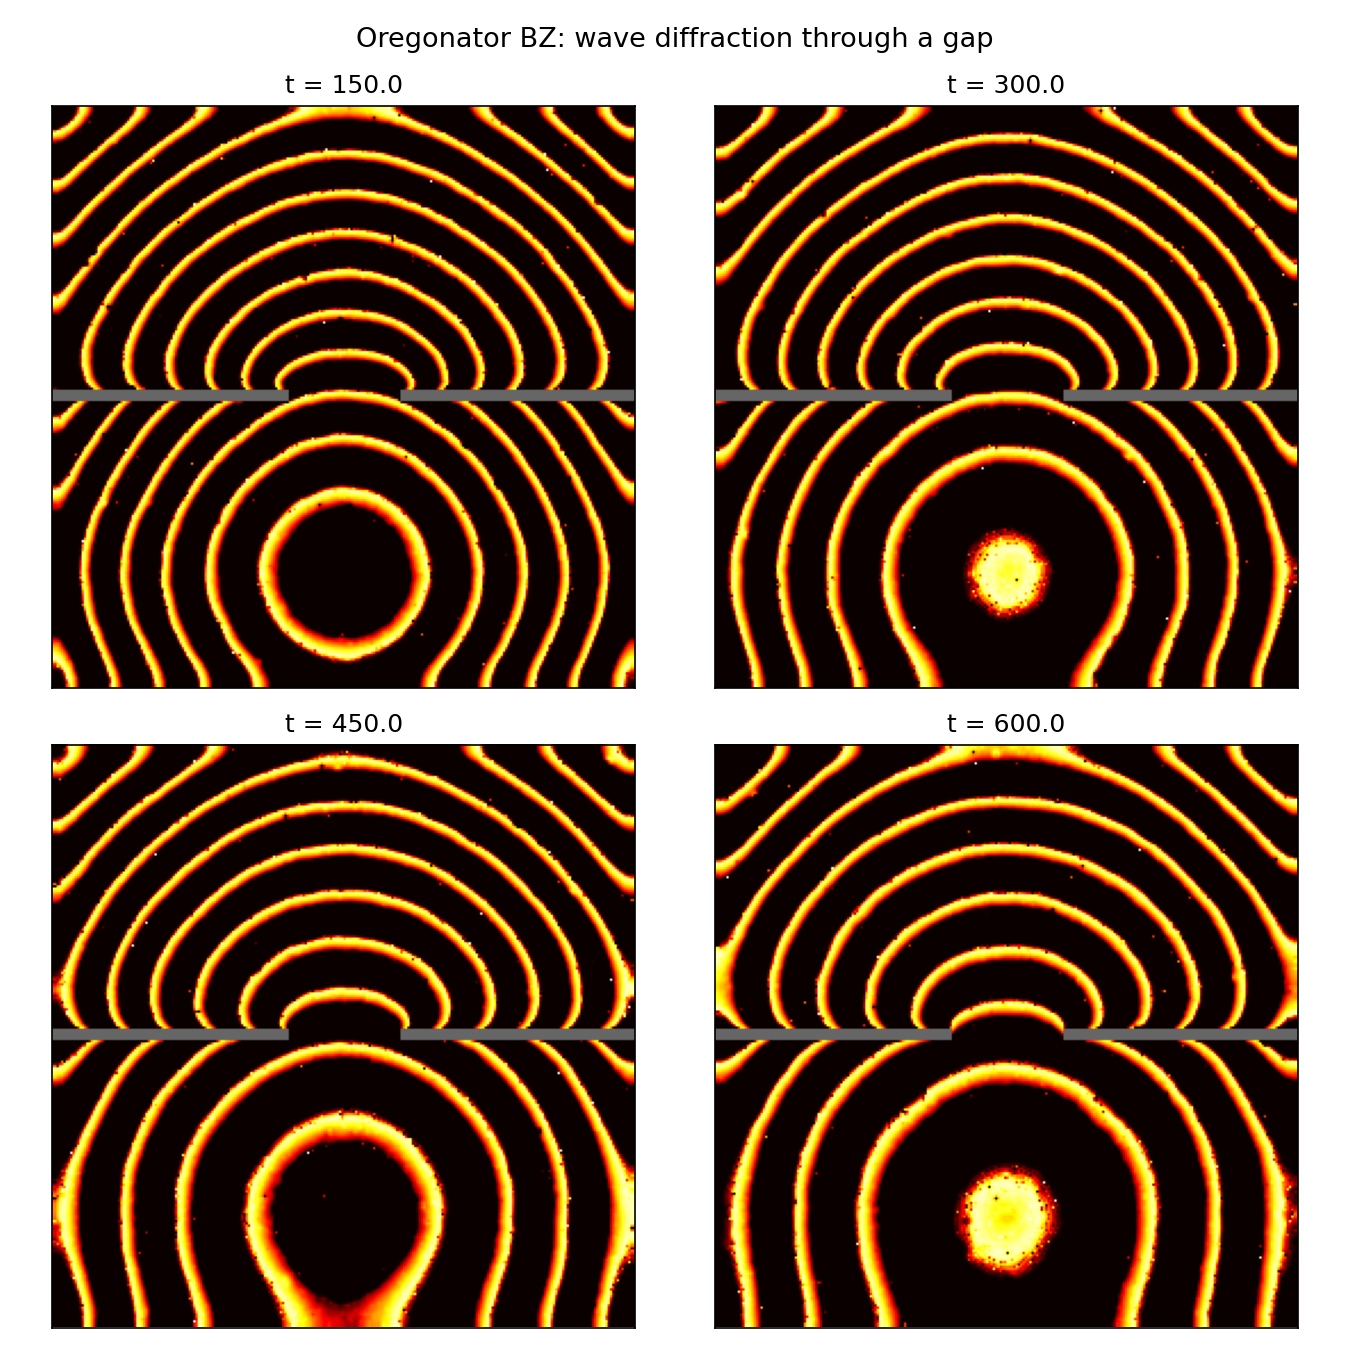
\includegraphics[width=0.55\textwidth]{../Analysis/oregonator_gap_diffraction.png}

\vspace{0.2cm}
\footnotesize
Next step: design a channel network so that input pulses are steered to the correct output port.

\end{frame}

% ---------------------------------------------------------------------
\begin{frame}{Next target: from free waves to channel routing}

\begin{columns}
\begin{column}{0.55\textwidth}
\textbf{Geometry:} no-flux walls form a channel network filled with BZ medium.

\vspace{0.2cm}
\textbf{Trainable knobs:}
\begin{itemize}
    \item wall positions / obstacle shapes,
    \item spatial catalyst density (tunes excitability),
    \item input timing, location, and amplitude.
\end{itemize}

\vspace{0.2cm}
\textbf{First task:} pulse routing.
\begin{itemize}
    \item Input at port 1 \textrightarrow{} high readout at output A.
    \item Input at port 2 \textrightarrow{} high readout at output B.
\end{itemize}

\vspace{0.2cm}
\textbf{Then:} train annihilation at a merge so both inputs give low output \textrightarrow{} XOR-like behaviour.
\end{column}

\begin{column}{0.40\textwidth}
\centering
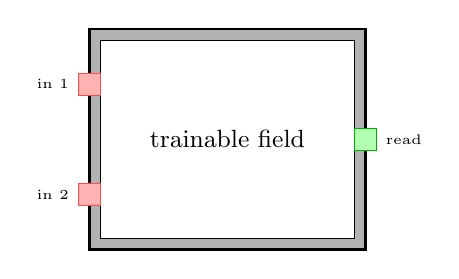
\begin{tikzpicture}[scale=0.7,
    wall/.style={draw=black, fill=black!30, line width=1pt},
    port/.style={draw=red!70, fill=red!30, minimum width=8pt, minimum height=8pt},
    probe/.style={draw=green!70!black, fill=green!30, minimum width=8pt, minimum height=8pt}]

\draw[wall] (0,0) rectangle (5,4);
\draw[fill=white] (0.2,0.2) rectangle (4.8,3.8);
\node[port] at (0,1) {};
\node[port] at (0,3) {};
\node[probe] at (5,2) {};
\node[left] at (-0.2,1) {\tiny in 2};
\node[left] at (-0.2,3) {\tiny in 1};
\node[right] at (5.2,2) {\tiny read};
\node at (2.5,2) {\small trainable field};
\end{tikzpicture}
\end{column}
\end{columns}

\end{frame}

% ---------------------------------------------------------------------
\begin{frame}{How we will train the geometry / field}

\begin{enumerate}
    \item \textbf{Parameterise the design.}
    \begin{itemize}
        \item Low-dim: positions/sizes of a few obstacles.
        \item High-dim: pixel-wise $F(x,y)$, $k(x,y)$ fields.
    \end{itemize}
    \item \textbf{Forward solve} the RD PDE for each candidate design.
    \item \textbf{Define a loss} on the readout (e.g. MSE against target truth table).
    \item \textbf{Optimise} with L-BFGS-B (continuous params) or CMA-ES (rough/discrete landscape).
\end{enumerate}

\vspace{0.3cm}
This is the same in-silico training loop we already used for the well-mixed CRN, but now the state is a spatial field instead of a concentration vector.

\end{frame}

% ---------------------------------------------------------------------
\begin{frame}{Why this is better than the DNA route}

\begin{table}
\centering
\small
\begin{tabular}{p{4.5cm}cc}
\toprule
\textbf{Criterion} & \textbf{DNA WTA} & \textbf{RD + geometry} \\
\midrule
Matches Project~11 premise & Partially & Strongly \\
Spatial continuity & No & Yes \\
Trainable geometry / topology & No & Yes \\
Parallel independent streams & No & Yes \\
Specialist molecular knowledge needed & High & Low \\
Link to CFD / microfluidics & Weak & Strong \\
Experimental realizability & DNA lab & BZ / IAA / microfluidics \\
\bottomrule
\end{tabular}
\end{table}

\end{frame}

% ---------------------------------------------------------------------
\begin{frame}{What we need from this meeting}

\begin{enumerate}
    \item \textbf{Confirm the pivot:} Oregonator BZ reaction-diffusion in trainable geometry as the main direction.
    \item \textbf{Pick the first demo:} 1D pulse routing, 2D XOR in a channel, or colliding-wave gate?
    \item \textbf{Set the scope:} Oregonator now; full chemistry / light-sensitive variants later?
    \item \textbf{Trainable variables:} geometry only, or also the spatial light-suppression field $\phi(x,y)$?
    \item \textbf{Timeline check:} How much time do we have to produce results and write them up?
\end{enumerate}

\end{frame}

% ---------------------------------------------------------------------
\begin{frame}{Proposed work plan (next 2--4 weeks)}

\begin{enumerate}
    \item \textbf{Week 1 (done):} Oregonator BZ solver running; target waves, collision, and gap diffraction demonstrated.
    \item \textbf{Week 2:} Add channel walls and reproduce basic wave routing / annihilation in 2D.
    \item \textbf{Week 3:} train wall positions or $\phi(x,y)$ for a two-input logic gate.
    \item \textbf{Week 4:} Compare against a simple digital baseline; document physics and limitations.
\end{enumerate}

\vspace{0.3cm}
\centering
\textbf{If this works, we have a continuous, spatial, trainable computing primitive for Project~11.}

\end{frame}

% ---------------------------------------------------------------------
\begin{frame}{Conclusion}

\begin{itemize}
    \item We explored acoustic, well-mixed CRN, and DNA directions.
    \item The DNA route is elegant but does not match the Project~11 premise.
    \item BZ reaction-diffusion in designed geometry is a simpler, more physical, and more aligned path.
    \item We already have a 2D Oregonator BZ solver producing target waves, collision, and gap diffraction.
    \item Next step: constrain it with channel geometry and train the geometry / light field for wave routing / logic gates.
\end{itemize}

\vspace{0.4cm}
\centering
\textbf{We need a decision today on the direction.}

\end{frame}

% ---------------------------------------------------------------------
\begin{frame}{References}

{\footnotesize
\begin{enumerate}
    \item A. Dack \textit{et al.} Recurrent neural chemical reaction networks that approximate arbitrary dynamics. \textit{Cell Systems}, 2026.
    \item K. M. Cherry \& L. Qian. Scaling up molecular pattern recognition with DNA-based winner-take-all neural networks. \textit{Nature} 559, 370--376 (2018).
    \item A. Adamatzky \& B. De Lacy Costello. Experimental logical gates in a reaction-diffusion medium. \textit{Phys. Rev. E} 66, 046112 (2002).
    \item J. E. Pearson. Complex patterns in a simple system. \textit{Science} 261, 189--192 (1993).
    \item T. Tóth \& K. Showalter. Logic gates in excitable media. \textit{J. Chem. Phys.} 103, 2058 (1995).
\end{enumerate}
}

\end{frame}

\end{document}
